\documentclass{article} % For LaTeX2e
\usepackage{nips13submit_e,times}
\usepackage{hyperref}
\usepackage{epsfig}
%\usepackage{mahnig}
\usepackage{url}
\usepackage{enumerate}
\usepackage{booktabs}
%\documentstyle[nips13submit_09,times,art10]{article} % For LaTeX 2.09
\usepackage{multicol}


\title{Shape classification using supervised classifiers}

\author{Julen Etxaniz and Ibon Urbina}

% The \author macro works with any number of authors. There are two commands
% used to separate the names and addresses of multiple authors: \And and \AND.
%
% Using \And between authors leaves it to \LaTeX{} to determine where to break
% the lines. Using \AND forces a linebreak at that point. So, if \LaTeX{}
% puts 3 of 4 authors names on the first line, and the last on the second
% line, try using \AND instead of \And before the third author name.

\newcommand{\fix}{\marginpar{FIX}}
\newcommand{\new}{\marginpar{NEW}}

\nipsfinalcopy % Uncomment for camera-ready version

\begin{document}

\maketitle

\begin{abstract}
In this document we report our proposal for the application of supervised classification methods to the shape classification problem. The datasets we have selected are plane and car shapes. The classifiers that we have selected for the classification tasks were: Decision Trees, Linear discriminant analysis and Logistic regression. We have implemented the classification process primarily using the scikit-learn and pandas library. We have learned the classifiers using the train data and computed the accuracy in the test data. We have performed several additional tasks: scaling, feature selection, feature engineering and pipeline optimization. On the one hand, we have concluded that the best option for plane data is Random Forest feature selection and LDA classifier. On the other hand, the best option for car data is LDA feature engineering and LDA classifier.
\end{abstract}

\tableofcontents
\newpage

\section{Description of the problem}
The task we have to solve is the classification of the shape datasets, introduced in \cite{Thakoor:2007} \cite{Thakoor:2005-July} \cite{Thakoor:2005-Oct} and available in \url{http://biomecis.uta.edu/shape_data.htm}. 
 
There are 4 shape datasets available. We have selected the plane and car datasets. In each dataset, shapes are represented as Cartesian coordinates of each point on the perimeter; all stored as MATLAB data files named as $Class\%d\_Sample\%d.mat$.

\subsection{Plane dataset}

Shape database was created by taking 640X480 resolution pictures of replica models of airplanes from top.
The plane dataset has the following characteristics:

\begin{itemize}
    \item $890*2+1=1781$ features. The minimum x and y values and perimeter length.
    \item $7$ classes: (a) Mirage, (b) Eurofighter, (c) F-14 wings closed, (d) F-14 wings opened, (e) Harrier, (f) F-22, (g) F-15. See Figure \ref{fig:plane}.
    \item $210$ instances. 
    \item The data is perfectly balanced. There are 30 instances in each class.
\end{itemize}

\begin{figure}[ht]
    \centering
    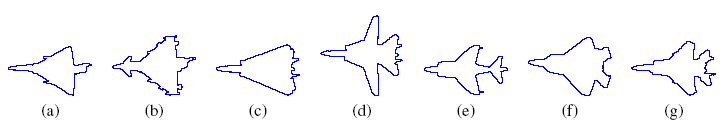
\includegraphics[width=\linewidth]{shape_plane.png}
    \caption{$7$ plane classes: (a) Mirage, (b) Eurofighter, (c) F-14 wings closed, (d) F-14 wings opened, (e) Harrier, (f) F-22, (g) F-15.}
    \label{fig:plane}
\end{figure}

\subsection{Car dataset}

Approach discussed in \cite{Thakoor:2005-Sept} was applied to 320X240 resolution videos to extract these shapes. As object extraction approach does not deal with shadows, the shapes are distorted in the bottom half. Samples show larger within-class variation, because vehicles of different makes and models vary.
The car dataset has the following characteristics:

\begin{itemize}
    \item $272*2+1=545$ features. The minimum x and y values and perimeter length.
    \item $4$ classes: (a) Sedan, (b) Pickup, (c) Minivan, (d) SUV. See Figure \ref{fig:car}.
    \item $120$ instances. 
    \item The data is perfectly balanced. There are 30 instances in each class.
\end{itemize}

\begin{figure}[ht]
    \centering
    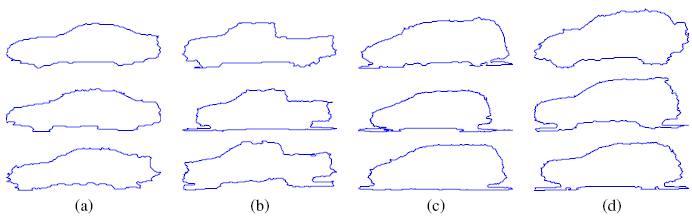
\includegraphics[width=\linewidth]{shape_car.png}
    \caption{$4$ car classes: (a) Sedan, (b) Pickup, (c) Minivan, (d) SUV.}
    \label{fig:car}
\end{figure}

\section{Description of our approach}
  
We organized the implementation of the project according to the tasks:

\begin{multicols}{2}
\begin{enumerate} 
    \item Importing the libraries
    \item Reading the datasets
    \item Preprocessing the datasets
    \item Scaling the data
    \item Dividing train and test data
    \item Classification
    \item Validation
    \item Feature Selection
    \item Feature Extraction
    \item Pipeline Optimization
\end{enumerate}
\end{multicols}

\subsection{Importing the libraries}

We import all the necessary libraries. Firstly, we used scipy.io.loadmat to read the dataset. Next, we used \textit{pandas} and numpy for preprocessing the dataset, and scikit-learn for the classification tasks. Moreover, we used matplotlib for viasualization. Finally, we used TPOT for pipeline optimization.

\subsection{Reading the datasets}

The main problem of both plane and car datasets is that each sample is a MATLAB file, which makes it to be only visible in MATLAB. To solve this, we use a helper function from the scipy.io package called loadmat which makes the data readable in python.

\subsection{Preprocessing}

We used the pandas library to represent the datasets as dataFrames. This structure makes the data flexible, easy to manipulate and good looking. 

The main problem of both plane and car datasets is that each sample is a MATLAB file, which makes it to be only visible in MATLAB. To solve this, we use a helper function from the scipy.io package called loadmat which makes the data readable in python. 

First, we collected the data in python lists and then transferred them to pandas DataFrame. When loading data with loadmat function it includes some information such as header, version and globals that is not useful for our classification; thus, we dropped them from the dataFrame. 

As we mention before, the only data available in each shape sample are the points that conform the perimeter. It is not mentioned to what class corresponds that data. This has to be taken from the file name which is a string concatenation of: Class + class number + Sample + sample number + .mat. 

Finally, to finish with the dataFrame representation, 1) we added perimeter length feature and 2) decided to change the way the points on the perimeter were described. Regarding to the first one, we thought that normalizing each sample array to the minimum perimeter length found in each dataset would make a more consistent and organized data: in the plane dataset the minimum perimeter corresponds to a sample formed by 890 and in the car dataset, corresponds to 272 points. Of course, doing this, the original length of the perimeter is lost; so, before resizing it, we stored the perimeter in a feature called Perimeter length.

On the other hand, the feature responsible for structuring the points on the perimeter is a single list containing one list for each sample that once again, contains a list of two numbers to represent a concrete point. The first number corresponds to the axis x and the second one to the axis y. Taking into account that in principle features must be unique values (either number or strings) and not lists, our structure is not a valid input for the classifiers when fitting them. In this situation, we made the decision of making one feature per axis value. So, if one sample is defined with this unique feature: [[x1, x2], [x2, y2], ..., [xn, yn]]. Now, is going to be defined by n*2 features: [x1, y1, x2, y2, ..., xn, yn].

\subsection{Scaling the data}
 
We scaled the data using $StandardScaler$. This scaler standardizes features by removing the mean and scaling to unit variance. Scaling the data before classification is recommended for some classifiers because their performance is better.

Parameters:
\begin{multicols}{2}
\begin{itemize}
\item copy=True
\item with\_mean=True
\item with\_std=True
\end{itemize}
\end{multicols}

\subsection{Dividing train and test data}
 
The data was split into two different sets of the same length: train and test; even numbers for the first one and odd ones for the second. Again both sets are divided in two: features (perimeter length, axes x and axes y) and targets(the corresponding class of each sample). 

Train and data sets are essential for the classifier. The first one is used in the learning process and the second one in the measure of its performance.

\subsection{Classification}

We used three different classifiers. The parameters that are different from default are in \textbf{bold}.

\begin{enumerate}
    \item Decision trees with parameters:
    \begin{multicols}{2}
    \begin{itemize}
        \item criterion=’gini’
        \item splitter=’best’ 
        \item max\_depth=None 
        \item min\_samples\_split=2
        \item min\_samples\_leaf=1 
        \item min\_weight\_fraction\_leaf=0.0 
        \item max\_features=None 
        \item random\_state=None 
        \item max\_leaf\_nodes=None 
        \item min\_impurity\_decrease=0.0 
        \item min\_impurity\_split=None 
        \item class\_weight=None 
        \item presort=False
    \end{itemize}
    \end{multicols}
    \item Linear discriminant analysis with parameters:
    \begin{multicols}{2}
    \begin{itemize}
        \item solver=’svd’ 
        \item shrinkage=None 
        \item priors=None 
        \item n\_components=None 
        \item store\_covariance=False 
        \item tol=0.0001
    \end{itemize}
    \end{multicols}
    \item Logistic regression with parameters:
    \begin{multicols}{2}
    \begin{itemize}
        \item penalty=’l2’
        \item dual=False
        \item tol=0.0001
        \item C=1.0
        \item fit\_intercept=True
        \item intercept\_scaling=1
        \item class\_weight=None
        \item random\_state=None
        \item solver=’liblinear’
        \item \textbf{max\_iter=2000}
        \item multi\_class=’ovr’
        \item verbose=0, 
        \item warm\_start=False 
        \item n\_jobs=1
    \end{itemize}
    \end{multicols}
\end{enumerate}
 
\subsection{Validation}
 
To validate our results we computed the classifier accuracies in the test data for the three classifiers.

Another possibility was to compute the cross-validation in the complete dataset but we used the split between train and test because we assumed that either training and test data were sufficient. 

As an additional validation step we computed the confusion matrices for the three classifiers.
 
\subsection{Feature Selection}

We used feature selection to reduce the number of features. We had too many features, two features for each point in the contour perimeter, which makes a total number of 1781 features for the plane dataset: 2*890 (number of points in the perimeter) + 1 (the feature corresponding to the perimeter length) and 545 features for the car dataset: 2*272 (number of points in the perimeter) + 1 (the feature corresponding to the perimeter length). Remember that we have normalized each contour perimeter to the minimum length perimeter found in each dataset.

We used 2 different methods for feature selection: \textit{SelectKBest} and \textit{RandomForest}. Both being supervised methods as they use each feature list and corresponding labels. 

The parameters of \textit{SelectKBest}:
\begin{multicols}{2}
\begin{itemize}
    \item score\_func=f\_classif
    \item score\_func=f\_classif
    \item score\_func=f\_classif
    \item score\_func=f\_classif
    \item score\_func=f\_classif
    \item \textbf{k=100}
    \item \textbf{k=200}
    \item \textbf{k=300}
    \item \textbf{k=400}
    \item \textbf{k=500}
\end{itemize}
\end{multicols}

The parameters of \textit{RandomForest}:
\begin{multicols}{2}
\begin{itemize}
    \item \textbf{n\_estimators=1-60}
    \item criterion='gini'
    \item max\_depth=None
    \item min\_samples\_split=2
    \item min\_samples\_leaf=1
    \item min\_weight\_fraction\_leaf=0.0
    \item max\_features='auto'
    \item max\_leaf\_nodes=None
    \item min\_impurity\_decrease=0.0
    \item min\_impurity\_split=None
    \item bootstrap=True
    \item oob\_score=False
    \item n\_jobs=None
    \item random\_state=None
    \item verbose=0
    \item warm\_start=False
    \item class\_weight=None
    \item ccp\_alpha=0.0
    \item max\_samples=None
\end{itemize}
\end{multicols}

\subsection{Feature Engineering}

As mentioned above, our features length was a problem. Thus, we tried feature engineering for features dimensionality reduction. We extracted 3 feature so that we can plot them in 3 dimensions.

We used 2 different methods for feature engineering: \textit{PCA} and \textit{LDA}. The first one is an unsupervised technique as it tries to find the directions of maximal variances, while the second one attempts to find a features subspace that maximizes class separability. Logically, to separate one class from another needs to know the corresponding feature-class information, making it easier with supervised technique.

The parameters of PCA:
\begin{multicols}{2}
\begin{itemize}
    \item \textbf{n\_components=3}
    \item copy=True
    \item whiten=False
    \item svd\_solver='auto'
    \item tol=0.0
    \item iterated\_power='auto'
    \item random\_state=None
\end{itemize}
\end{multicols}

The parameters of LDA:
\begin{multicols}{2}
\begin{itemize}
    \item solver='svd'
    \item shrinkage=None
    \item priors=None
    \item \textbf{n\_components=3}
    \item store\_covariance=False
    \item tol=0.0001
\end{itemize}
\end{multicols}

\subsection{Pipeline Optimization}

We used TPOT to generate an optimal pipeline to compare its accuracy with ours. This way we can know how good our classifiers are. We can compare the accuracies obtained with TPOT with ours.

The parameters of the TPOT classifier:
\begin{multicols}{2}
\begin{itemize}
    \item \textbf{generations=5}
    \item \textbf{population\_size=10}
    \item offspring\_size=None 
    \item mutation\_rate=0.9
    \item crossover\_rate=0.1
    \item scoring='accuracy'
    \item cv=5
    \item subsample=1.0
    \item n\_jobs=1
    \item max\_time\_mins=None
    \item max\_eval\_time\_mins=5
    \item \textbf{random\_state=16}
    \item config\_dict=None
    \item template=None
    \item warm\_start=False
    \item memory=None
    \item use\_dask=False
    \item periodic\_checkpoint\_folder=None
    \item early\_stop=None
    \item \textbf{verbosity=2}
    \item disable\_update\_check=False
    \item log\_file=None
\end{itemize}
\end{multicols}
 
\section{Implementation}

All the project steps were implemented in Python. Firstly, we used scipy.io.loadmat to read the dataset. Next, we used \textit{pandas} and numpy for preprocessing the dataset, and scikit-learn for the classification tasks. Moreover, we used matplotlib for viasualization. Finally, we used TPOT for pipeline optimization.

We illustrate how the implementation works with explanations in the Jupyter notebook \texttt{P59\_Shape\_Classification\_ML\_D2.ipynb}. In most of the cases, we defined the functions first and then used them. This avoids repeating the code in different steps or on the same step with different datasets. The project description, the notebook, the dataset and the written report are available at \url{https://github.com/juletx/shape-classification-ml}.

\section{Results}

\subsection{Not scaled data}

\subsubsection{Plane dataset}

The accuracies produced by the Decision tree, LDA and Logistic regression classifiers were, respectively: $0.7714$, $0.9523$, and $0.9428$. Therefore, the best classifier for not scaled plane data was LDA. Decision tree obtains a very low accuracy compared to the other two.

The results of the computation of the confusion matrices for Decision tree, LDA and Logistic regression classifiers are respectively shown in Tables \ref{tab:CM_PLANE_DT}, \ref{tab:CM_PLANE_LDA}, and \ref{tab:CM_PLANE_LR}.

The analysis of the confusion matrices shows that the most difficult discrimination is for the first 2 classes, Mirage and Eurofighter. This occurs because they are mistaken with other planes. For example, the Eurofighter is commonly mistaken with F-15.

\begin{table}
\centering
\begin{tabular}{lrrrrrrr}
\toprule
col\_0 &  1 &  2 &   3 &   4 &   5 &   6 &   7 \\
Class &    &    &     &     &     &     &     \\
\midrule
1     &  7 &  2 &   2 &   1 &   0 &   1 &   2 \\
2     &  2 &  8 &   0 &   0 &   1 &   0 &   4 \\
3     &  1 &  1 &  10 &   0 &   0 &   2 &   1 \\
4     &  0 &  1 &   0 &  14 &   0 &   0 &   0 \\
5     &  0 &  0 &   0 &   0 &  14 &   1 &   0 \\
6     &  0 &  0 &   0 &   0 &   0 &  15 &   0 \\
7     &  2 &  0 &   0 &   0 &   0 &   0 &  13 \\
\bottomrule
\end{tabular}
\caption{Confusion matrix produced by the Decision tree classifier on plane data}
\label{tab:CM_PLANE_DT}
\end{table}

\begin{table}
\centering
\begin{tabular}{lrrrrrrr}
\toprule
col\_0 &   1 &   2 &   3 &   4 &   5 &   6 &   7 \\
Class &     &     &     &     &     &     &     \\
\midrule
1     &  13 &   0 &   0 &   0 &   0 &   2 &   0 \\
2     &   0 &  12 &   0 &   0 &   0 &   0 &   3 \\
3     &   0 &   0 &  15 &   0 &   0 &   0 &   0 \\
4     &   0 &   0 &   0 &  15 &   0 &   0 &   0 \\
5     &   0 &   0 &   0 &   0 &  15 &   0 &   0 \\
6     &   0 &   0 &   0 &   0 &   0 &  15 &   0 \\
7     &   0 &   0 &   0 &   0 &   0 &   0 &  15 \\
\bottomrule
\end{tabular}
\caption{Confusion matrix produced by the LDA classifier on plane data}
\label{tab:CM_PLANE_LDA}
\end{table}

\begin{table}
\centering
\begin{tabular}{lrrrrrrr}
\toprule
col\_0 &   1 &   2 &   3 &   4 &   5 &   6 &   7 \\
Class &     &     &     &     &     &     &     \\
\midrule
1     &  13 &   0 &   1 &   0 &   0 &   1 &   0 \\
2     &   1 &  11 &   0 &   0 &   0 &   0 &   3 \\
3     &   0 &   0 &  15 &   0 &   0 &   0 &   0 \\
4     &   0 &   0 &   0 &  15 &   0 &   0 &   0 \\
5     &   0 &   0 &   0 &   0 &  15 &   0 &   0 \\
6     &   0 &   0 &   0 &   0 &   0 &  15 &   0 \\
7     &   0 &   0 &   0 &   0 &   0 &   0 &  15 \\
\bottomrule
\end{tabular}
\caption{Confusion matrix produced by the Logistic regression classifier on plane data}
\label{tab:CM_PLANE_LR}
\end{table}

\subsubsection{Car dataset}

The accuracies produced by the Decision tree, LDA and Logistic regression classifiers were, respectively: $0.7833$, $0.9000$, and $0.8666$. Therefore, the best classifier for not scaled car data was LDA.

The results of the computation of the confusion matrices for Decision tree, LDA and Logistic regression classifiers are respectively shown in Tables \ref{tab:CM_CAR_DT}, \ref{tab:CM_CAR_LDA}, and \ref{tab:CM_CAR_LR}.

The analysis of the confusion matrices shows that there are more differences between classifiers. Decision tree for example has by far the most problems with class 4. The others classifiers make less mistakes but we can also see slight differences between classes.

\begin{table}
\centering
\begin{tabular}{lrrrr}
\toprule
col\_0 &   1 &   2 &   3 &  4 \\
Class &     &     &     &    \\
\midrule
1     &  13 &   0 &   0 &  2 \\
2     &   0 &  13 &   1 &  1 \\
3     &   0 &   0 &  15 &  0 \\
4     &   0 &   7 &   2 &  6 \\
\bottomrule
\end{tabular}
\caption{Confusion matrix produced by the Decision tree classifier on car data}
\label{tab:CM_CAR_DT}
\end{table}

\begin{table}
\centering
\begin{tabular}{lrrrr}
\toprule
col\_0 &   1 &   2 &   3 &   4 \\
Class &     &     &     &     \\
\midrule
1     &  13 &   0 &   0 &   2 \\
2     &   0 &  15 &   0 &   0 \\
3     &   0 &   1 &  13 &   1 \\
4     &   0 &   0 &   2 &  13 \\
\bottomrule
\end{tabular}
\caption{Confusion matrix produced by the LDA classifier on car data}
\label{tab:CM_CAR_LDA}
\end{table}

\begin{table}
\centering
\begin{tabular}{lrrrr}
\toprule
col\_0 &   1 &   2 &   3 &   4 \\
Class &     &     &     &     \\
\midrule
1     &  14 &   0 &   1 &   0 \\
2     &   0 &  14 &   1 &   0 \\
3     &   0 &   1 &  12 &   2 \\
4     &   0 &   0 &   3 &  12 \\
\bottomrule
\end{tabular}
\caption{Confusion matrix produced by the Logistic regression classifier on car data}
\label{tab:CM_CAR_LR}
\end{table}

\subsection{Scaled data}

The accuracies produced by the Decision tree, LDA and Logistic regression classifiers were, respectively: $0.7809$, $0.9523$, and $0.9238$. Therefore, the best classifier for scaled plane data was LDA. We can see that the accuracy for Decision tree increased, LDA is the same and Logistic regression decreased.

The accuracies produced by the Decision tree, LDA and Logistic regression classifiers were, respectively: $0.8333$, $0.9000$, and $0.9166$. Therefore, the best classifier for scaled car data was Logistic regression. We can see that the accuracy for Decision tree increased, LDA is the same and Logistic regression increased.

\subsection{Conclusions regarding to scaling or not scaling the data}
For our thoughts the results were kind of unexpected. We thought that scaling the data would be decisive regarding to improving the accuracy scores (things were not so decisive). However, best results in the plane dataset were given by the LDA classifier and match exactly with the percentage obtain from the scaled and not scaled data: $0.9523$. On the other hand, for the car dataset we obtained a better score with the scaled data; so here yes, our prognostic was succeed : $0.8666$ vs $0.9166$ in the Logistic regression classifier.

\subsection{Feature Selection}

\subsubsection{SelectKBest}

For this method, we decided to compute the accuracy evolution starting with 100 features and ending with 500. Each time, we summed up 100 features to the algorithm. This process was done either for scaled and not scaled data.

\textbf{Plane dataset}: accuracy scores regarding to the selected number of features \textbf{without scaling} them:
\begin{multicols}{2}
\begin{itemize}
    \item 100 features:
    \subitem DT: $0.5619$
    \subitem LDA: $0.2571$
    \subitem LR: $0.6190$
    \item 200 features
    \subitem DT: $0.6761$
    \subitem LDA: $0.4952$
    \subitem LR: $0.6285$
    \item 300 features
    \subitem DT: $0.7333$
    \subitem LDA: $0.7047$
    \subitem LR: $0.7047$
    \item 400 features
    \subitem DT: $0.7523$
    \subitem LDA: $0.7714$
    \subitem LR: $0.8190$
    \item 500 features
    \subitem DT: $0.7142$
    \subitem LDA: $0.7809$
    \subitem LR: $0.8761$
\end{itemize}
\end{multicols}

\textbf{Plane dataset}: accuracy scores regarding to the selected number of features \textbf{scaling} them:
\begin{multicols}{2}
\begin{itemize}
    \item 100 features:
    \subitem DT: $0.5047$
    \subitem LDA: $0.2571$
    \subitem LR: $0.6190$
    \item 200 features
    \subitem DT: $0.6571$
    \subitem LDA: $0.4952$
    \subitem LR: $0.6285$
    \item 300 features
    \subitem DT: $0.7238$
    \subitem LDA: $0.7047$
    \subitem LR: $0.7047$
    \item 400 features
    \subitem DT: $0.7619$
    \subitem LDA: $0.7714$
    \subitem LR: $0.8190$
    \item 500 features
    \subitem DT: $0.7333$
    \subitem LDA: $0.7809$
    \subitem LR: $0.8761$
\end{itemize}
\end{multicols}

\textbf{Car dataset}: accuracy scores regarding to the selected number of features \textbf{without scaling} them:
\begin{multicols}{2}
\begin{itemize}
    \item 100 features:
    \subitem DT: $0.7666$
    \subitem LDA: $0.4333$
    \subitem LR: $0.6$
    \item 200 features
    \subitem DT: $0.8333$
    \subitem LDA: $0.6666$
    \subitem LR: $0.7166$
    \item 300 features
    \subitem DT: $0.8166$
    \subitem LDA: $0.8333$
    \subitem LR: $0.8833$
    \item 400 features
    \subitem DT: $0.8666$
    \subitem LDA: $0.8666$
    \subitem LR: $0.85$
    \item 500 features
    \subitem DT: $0.85$
    \subitem LDA: $0.8833$
    \subitem LR: $0.8666$
\end{itemize}
\end{multicols}

\textbf{Car dataset}: accuracy scores regarding to the selected number of features \textbf{scaling} them:
\begin{multicols}{2}
\begin{itemize}
    \item 100 features:
    \subitem DT: $0.7833$
    \subitem LDA: $0.4333$
    \subitem LR: $0.6$
    \item 200 features
    \subitem DT: $0.8166$
    \subitem LDA: $0.6666$
    \subitem LR: $0.7166$
    \item 300 features
    \subitem DT: $0.75$
    \subitem LDA: $0.8333$
    \subitem LR: $0.8833$
    \item 400 features
    \subitem DT: $0.8333$
    \subitem LDA: $0.8666$
    \subitem LR: $0.85$
    \item 500 features
    \subitem DT: $0.75$
    \subitem LDA: $0.8833$
    \subitem LR: $0.8666$
\end{itemize}
\end{multicols}

\subsection{Conclusions regarding to SelectKBest algorithm}

The main conclusion we reach in this process is that not always more features implies better accuracy scores; it depends also, for example, in the classifier you are using. If we take a look in the accuracy score (plane datases + not scaled) and observe the scores obtained with 300 features and 500 features in the decision tree classifier, we see that with less features it obtains an accuracy of $0.7333$ and with 500, $0.7142$. But, for the logistic regression classifier, with 300 features obtain a $0.7047$ and with 500, $0.8761$.

\subsubsection{RandomForest}

RandomForest is a good algorithm for feature selection. As we see in the theorical classes, the algorithm to learn decision trees adopts a greedy divide-and-conquer strategy selecting always the most important attribute first. The most important attribute is the one that makes the most important difference to the classification; and this, is usually measured by a rank where the features make the maximal impurity decrease.

However, there is no way to know fully certain which is the number of trees that makes the best feature selection. The reason behind this is that RandomForest is an ensemble of decision trees; each one learned on a bootstrap sample. This means that each bootstrap sample is computed using a subset of features/variables that are selected randomly each time.

To avoid this and quantify the best performance for the number of trees used when selecting the features that make the best accuracy score, we measured ten different trials. Each trial, consisted on selecting from 1 to 60 the number of trees used and then, computing the accuracy scores. All this is constrained by a condition: we are able to to sum up one tree to the current tree numbers parameter if the current selected number of trees has obtained a better accuracy score than the previous numbers of trees obtained. In each trial, the obtained maximum accuracy score, the name of the classifier with which we obtain that score and the number of features used to obtain the maximum scores were taken.

\textbf{Plane dataset, not scaled}: results regarding to the RandomForest algorithm (making a mean of the 10 trials):
\begin{itemize}
    \item More often appeared classifier: LDA
    \item Mean number of used trees: 8
    \item Mean number of used features: 81
    \item Mean accuracy score: $0.9637$
\end{itemize}

\textbf{Car dataset, not scaled}: results regarding to the RandomForest algorithm (making a mean of the 10 trials):
\begin{itemize}
    \item More often appeared classifier: LG
    \item Mean number of used trees: 6
    \item Mean number of used features: 44
    \item Mean accuracy score: $0.8833$
\end{itemize}

For both datasets it was worth using RandomForest feature section process against SelectKBest algorithm, as it obtained better ratio regarding to selected/used features and accuracy scores.

\subsection{Feature Engineering}

\subsubsection{PCA}

The accuracies produced by the LDA classifier on PCA reduced plane data was $0.6190$. The accuracy obtained is much lower to using all features. Therefore, PCA is not a good option for feature engineering or dimensionality reduction.

The accuracies produced by the LDA classifier on PCA reduced car data was $0.5166$. The accuracy obtained is much lower to using all features. Therefore, PCA is not a good option for feature engineering or dimensionality reduction.

\subsubsection{LDA}

The accuracies produced by the LDA classifier on LDA reduced plane data were $0.9333$ and $0.9523$ for not scaled and scaled data, respectively. The accuracy obtained is similar to using all features. Therefore, PCA is a good option for feature engineering or dimensionality reduction.

The accuracies produced by the LDA classifier on LDA reduced car data was $0.9000$ and $0.9000$ for not scaled and scaled data, respectively. The accuracy obtained is similar to using all features. Therefore, PCA is a good option for feature engineering or dimensionality reduction.

\subsection{Pipeline Optimization}

We have realised that TPOT produces different results sometimes and we know that the produced pipeline is not always the optimal. But, we think that it is still interesting to have an idea of how good our solution is.

The best internal CV score of the pipeline obtained by TPOT on the \textbf{plane data} was $0.9714$. The accuracy on test data was $0.9142$. The pipeline we obtained was: 

[('linearsvc', LinearSVC(C=25.0, dual=False, random\_state=16, tol=1e-05))]

The accuracy obtained is a lot lower than our best option. So, we can say that our classifier is very good.

The best internal CV score of the pipeline obtained by TPOT on the \textbf{car data} was $0.8166$. The accuracy on test data was $0.9166$. The pipeline we obtained was: 

[('gradientboostingclassifier',
  GradientBoostingClassifier (learning\_rate=0.5, max\_depth=4, max\_features=0.4,
                             min\_samples\_leaf=5, min\_samples\_split=8,
                             random\_state=16, subsample=0.5))]

The accuracy obtained is a bit higher than our best option. So, we can say that our classifier is quite good.

\section{Conclusions}

As you may see, we have made a huge experiment trying out different algorithms regarding to data preprocessing, classifiers, feature selection and feature engineering. For example, at first we obtained lower accuracies after feature selection and engineering. So, we had to try different options to improve the accuracy. 

In general, results were quite good, but the accuracy for car data was significantly lower. We think that the reason for obtaining a lower accuracy in the car data is that the images are more similar and distorted. We also saw that even if the datasets are similar the best solution is not the same.

For our databases and used algorithms, this is the best solution combination we found:

For the \textbf{plane dataset}:
\begin{itemize}
    \item Not scaled data
    \item Feature selection: Random Forest
    \subitem Number of trees: 8
    \subitem Number of features: 81
    \item Classifier: Linear Discriminant Analysis
    \item Mean accuracy score: $0.9637$
\end{itemize}

For the \textbf{car dataset}:
\begin{itemize}
    \item Not scaled data
    \item Feature engineering: LDA
    \item Classifier: Linear Discriminant Analysis
    \item Mean accuracy score: $0.9000$
\end{itemize}

\bibliographystyle{unsrt}
\bibliography{bibtex_references_project}

\end{document}
